\documentclass[10pt]{jarticle}
\usepackage[dvipdfmx]{graphicx}
\usepackage{amsmath}
\usepackage{comment}
\usepackage{setspace}
\usepackage{float}
\usepackage{indentfirst}
\usepackage{here}
\usepackage{caption}
\usepackage{multicol}

\captionsetup[figure]{font=footnotesize}

\setlength{\hoffset}{0cm}
\setlength{\oddsidemargin}{-15mm}
\setlength{\evensidemargin}{-3cm}
\setlength{\marginparsep}{0cm}
\setlength{\marginparwidth}{0cm}
\setlength{\textheight}{26.7cm}
\setlength{\textwidth}{19cm}
\setlength{\topmargin}{-50pt}      % 上の余白を調整
\setlength\abovecaptionskip{0pt}

\renewcommand{\baselinestretch}{1.0}
\renewcommand{\floatpagefraction}{1}
\renewcommand{\topfraction}{1}
\renewcommand{\bottomfraction}{1}
\renewcommand{\textfraction}{0}
\renewcommand{\labelenumi}{(\arabic{enumi})}
\renewcommand{\figurename}{Fig.} %図をFig.にする(画像のとこだけ)

\begin{comment}
  %図のキャプションからコロン:を消す
  \makeatletter
  \long\def\@makecaption#1#2{% #1=図表番号,#2=キャプション本文
    \sbox\@tempboxa{#1. #2}
    \ifdim \wd\@tempboxa >\hsize
    #1 #2\par 
    \else
    \hb@xt@\hsize{\hfil\box\@tempboxa\hfil}
    \fi
  }  
  \makeatother 
\end{comment}

%%sectionの前後の余白を消す
\makeatletter
\def\section{\@startsection {section}{1}{\z@}{-0.5ex plus -1ex minus -.2ex}{0.5 ex plus .2ex}{\small\bf}}
\def\subsection{\@startsection {subsection}{1}{\z@}{-0.5ex plus -1ex minus -.2ex}{0.5 ex plus .2ex}{\small\bf}}
\def\subsubsection{\@startsection {subsubsection}{1}{\z@}{-0.5ex plus -1ex minus -.2ex}{0.5 ex plus .2ex}{\footnotesize\bf}}
\makeatother

\pagestyle{myheadings}
%\pagestyle{empty} % すべてのページ番号を消去

\begin{document}

%文字サイズ
%\scriptsize   %7pt
\footnotesize %8pt
%\small        %9pt


%% <------------------------------タイトル------------------------------>

\markright{第  回全日本学生フォーミュラ大会 Car No.000 **大学デザインレポート}

\date{\vspace{-15mm}}
\title{\vspace{-18mm} \small Car No.000 [team name] Design Report}

\oddsidemargin = -15mm
\maketitle % 実際の表題の出力
\thispagestyle{empty}

%% <------------------------------ 本文 ------------------------------>

%イントロ
昨年度のKIT-formulaでは,2017年度大会において総合32位という結果に終わり,目標としていた歴代最高順位の8位を超える6位入賞を達成することが出来なかった.
したがって今年度では,根本的な車両の成り立ちを見直し,昨年度車両(以下KS-14)よりも確実に速く,勝てる車両を目指した.
そこで今年度の車両コンセプトを,昨年度よりも数段速い車両を意味し,また新たなことに挑戦するというチームの想いを込めた「Speed Evolution」とし,シングルナンバー(総合順位一桁)を目標に今年度車両(以下KS-15)の開発を行った.


\begin{multicols}{2} %%2列スタイル化
  
%コンセプト
%%%%%%%%%%%%%%%%%%%%%%%%%%%
\section{車両開発方針}
%%%%%%%%%%%%%%%%%%%%%%%%%%%
車両開発の目標であるシングルナンバーを獲得するため,動的競技のうち最も総合順位との相関のあるエンデュランスに着目した.過去3年の大会結果から,総合順位一桁のチームはエンデュランスにおいても高順位であることが分かった.そこで昨年度の結果から,エンデュランス総合タイムが1320 sec(平均タイム66.0 sec/lap)で総合順位が8位以上を獲得できることが分かったため,これを車両開発目標に設定し開発を行った.

%%%%%%%%%%%%%%%%%%%%%%%%%%%
\subsection{ベンチマーク分析}
%%%%%%%%%%%%%%%%%%%%%%%%%%%
前項にて設定したエンデュランス総合タイムで走行していた2017年度大会の他大学車両と,KS-14との間でどういった区間でタイム差が生じているかをベンチマークとして,昨年度大会の動画から検証を行った.動画から区間A,Bを設定し(区間A:高速状態での加速性能,旋回性能が重視される区間,区間B:低速からの加速性能,応答性能が重視される区間)分析を行ったところ,区間Aでは平均して$\Delta$1.557 sec,区間Bでは$\Delta$2.379 secと,KS-14とベンチマークとの間に差があることが分かった.そこでパワートレインでは主にエンジン低回転領域からの加速性能,サスペンションでは旋回性能に加え応答性能を重視して開発を行った.またフレームやエアロデバイスといったボディではサスペンションの性能要求を満たすこと,コクピットにおいては従来のDrivabilityに加え,今まで重要視していなかったドライバーの快適性(以下Comfortability)を追求することとした.またサスペンションからの性能要求を満たすため,各パーツにおいて軽量化の検討を行った.


%サスペンション
%%%%%%%%%%%%%%%%%%%%%%%%%%%
\section{サスペンション}
%%%%%%%%%%%%%%%%%%%%%%%%%%%
チーム目標であるシングルナンバーを獲得するためにサスペンション系では前述のコース,タイム分析からコーナーの定常領域で0.54 sec,過渡領域であるパイロンスラロームにおいて1.84 secの短縮が必要であることが分かった.

%suspension
%%%%%%%%%%%%%%%%%%%%%%%%%%%
\subsection{subtitle}
%%%%%%%%%%%%%%%%%%%%%%%%%%%
あいうえお(Fig.\ref{fig:label1}).

かきくけこ(Fig.\ref{fig:label2}).



%hubs
%%%%%%%%%%%%%%%%%%%%%%%%%%%
\section{title}
%%%%%%%%%%%%%%%%%%%%%%%%%%%
aaaaaaaaaaaaaa

%%%%%%%%%%%%%%%%%%%%%%%%%%%
\subsection{subtitle}
%%%%%%%%%%%%%%%%%%%%%%%%%%%
bbbbbbbbbbbbbb

%%%%%%%%%%%%%%%%%%%%%%%%%%%
\subsubsection{subsubtitle}
%%%%%%%%%%%%%%%%%%%%%%%%%%%
cccccccccccccc


%uplights
%%%%%%%%%%%%%%%%%%%%%%%%%%%
\section{title}
%%%%%%%%%%%%%%%%%%%%%%%%%%%
aaaaaaaaaaaaaa

%%%%%%%%%%%%%%%%%%%%%%%%%%%
\subsection{subtitle}
%%%%%%%%%%%%%%%%%%%%%%%%%%%
bbbbbbbbbbbbbb

%%%%%%%%%%%%%%%%%%%%%%%%%%%
\subsubsection{subsubtitle}
%%%%%%%%%%%%%%%%%%%%%%%%%%%
cccccccccccccc



%ボディ
%%%%%%%%%%%%%%%%%%%%%%%%%%%
\section{ボディ}
%%%%%%%%%%%%%%%%%%%%%%%%%%%
aaaaaaaaaaaaaaaaaaaaaaaa

%ボディ
%%%%%%%%%%%%%%%%%%%%%%%%%%%
\section{title}
%%%%%%%%%%%%%%%%%%%%%%%%%%%
aaaaaaaaaaaaaa

%%%%%%%%%%%%%%%%%%%%%%%%%%%
\subsection{subtitle}
%%%%%%%%%%%%%%%%%%%%%%%%%%%
bbbbbbbbbbbbbb

%%%%%%%%%%%%%%%%%%%%%%%%%%%
\subsubsection{subsubtitle}
%%%%%%%%%%%%%%%%%%%%%%%%%%%
cccccccccccccc


%エアロ
%%%%%%%%%%%%%%%%%%%%%%%%%%%
\section{title}
%%%%%%%%%%%%%%%%%%%%%%%%%%%
aaaaaaaaaaaaaa

%%%%%%%%%%%%%%%%%%%%%%%%%%%
\subsection{subtitle}
%%%%%%%%%%%%%%%%%%%%%%%%%%%
bbbbbbbbbbbbbb

%%%%%%%%%%%%%%%%%%%%%%%%%%%
\subsubsection{subsubtitle}
%%%%%%%%%%%%%%%%%%%%%%%%%%%
cccccccccccccc



%パワートレイン
%%%%%%%%%%%%%%%%%%%%%%%%%%%
\section{パワートレイン}
%%%%%%%%%%%%%%%%%%%%%%%%%%%
チーム目標を達成するためパワートレインのベンチマークよりも劣っている点を’17年度大会のエンデュランス区間タイムから分析を行った.
1.1項の分析の結果,低回転域からの加速性能がベンチマークよりも劣っていることが分かった.そこでパワートレインでは,更にその区間での分析を行い,1コーナーからストレートエンド到達までのタイム差がベンチマークよりも平均して0.4 sec遅く,最もタイムに影響を及ぼしていることに着目した.

ベンチマークでは上述の区間を60 mとすると,50 mを2.5 secで通過していることが分かった.従ってKS-15でのパワートレイン開発目標を,1コーナー脱出速度をロガーデータ等から40 km/hとし,「メインストレート50 mを2.5 secで走行可能な加速性能」とし開発を行った. 
またベンチマークの調査結果から,最高出力は最低80 PSを維持し,コーナー脱出時(低回転域)からの常用回転域でのトルク特性を重視した.常用回転域はKS-14のロガーデータ及びオンボード映像から5000~13000 rpmとした.

具体的には,まず吸気がKS-14の解析モデルをもとに設計を行い,それが終了次第排気が設計を行うという手順で行った.そして実走行において燃調セッティングにより解析値に近づける手法をとった.

%エンジン
%%%%%%%%%%%%%%%%%%%%%%%%%%%
\section{title}
%%%%%%%%%%%%%%%%%%%%%%%%%%%
aaaaaaaaaaaaaa

%%%%%%%%%%%%%%%%%%%%%%%%%%%
\subsection{subtitle}
%%%%%%%%%%%%%%%%%%%%%%%%%%%
bbbbbbbbbbbbbb

%%%%%%%%%%%%%%%%%%%%%%%%%%%
\subsubsection{subsubtitle}
%%%%%%%%%%%%%%%%%%%%%%%%%%%
cccccccccccccc


%吸気
%%%%%%%%%%%%%%%%%%%%%%%%%%%
\section{title}
%%%%%%%%%%%%%%%%%%%%%%%%%%%
aaaaaaaaaaaaaa

%%%%%%%%%%%%%%%%%%%%%%%%%%%
\subsection{subtitle}
%%%%%%%%%%%%%%%%%%%%%%%%%%%
bbbbbbbbbbbbbb

%%%%%%%%%%%%%%%%%%%%%%%%%%%
\subsubsection{subsubtitle}
%%%%%%%%%%%%%%%%%%%%%%%%%%%
cccccccccccccc


%排気
%%%%%%%%%%%%%%%%%%%%%%%%%%%
\subsection{排気}
%%%%%%%%%%%%%%%%%%%%%%%%%%%
排気系設計ではパワートレインの目標を達成するため常用回転域での更なるトルク向上と扱いやすい出力特性を目指し開発を行った.目標として常用回転域での最大軸トルクを60 N-mとした(前年度45N-m).加えて,ドライバーが扱いやすいリニアなトルク特性となるようにエンジンモデルを選定した.

またKS-14が孕んでいた様々な問題についても解決策を模索した.

%%%%%%%%%%%%%%%%%%%%%%%%%%%
\subsubsection{排気管}
%%%%%%%%%%%%%%%%%%%%%%%%%%%
まずKS-14の問題点として解析方法の未確立及び前年度との比較不足が挙げられた.これは,9月の段階にはGT-powerでKS-14のエンジンモデルを製作して解析を行い、比較対象を明確化することで解決した.次にKS-15では排気管の軽量化にも取り組み,排気系パーツ一つ一つの重量を実測・管理を徹底した.またKS-14から採用したはめ込み式の排気管は取り付けがしづらかったため,はめ込み式は踏襲しつつ集合部のみを一体形状とし整備性の向上に努めた.集合部は左右対称形状とすることで排気管の取り回し設計や製作を行いやすくした.またA/Fセンサーマウントを各気筒に配置することで,気筒別に燃調マッピングが行える構造とした.(Fig.\ref{fig:power3})

次に軸トルク向上及び扱いやすい出力特性を達成するため,吸気側が先に製作した’17年度エンジンモデルを参考に,主に排気管長と管径を変更しながら10個ほどのモデルを作成した.これらの解析結果から,管径よりも管長,特に集合部よりも前の管長(プライマリ)が出力特性に大きく影響を及ぼすことが分かった.そこで集合部以下を燃料タンクやフレームとの干渉を考慮しつつ必要最小限の管長・管径とした.管径については解析結果から僅かな差であるが$\phi$38.1が最適であったため,それ以降の解析は管長のみを変更し管径は常に$\phi$38.1で行った.以上の方法で約40個のモデルを作成し,その中から目標最大トルクを達成しかつリニアなトルク特性となるものを選定した.その結果プライマリ管長は495 mmとなった.Fig.\ref{fig:power4}にKS-14の標準バルブタイミングのものとKS-15のそれぞれのトルク・PS性能曲線を示す.Fig.\ref{fig:power4}から分かるように常用回転域において大幅にトルクが向上したことが分かる.また最大トルクは7500 rpmにおいて60.1 N-mとなり目標数値を達成した.また最小限の管長・管径としたことにより排気管で200 gの軽量化を実現することが出来た.

%%%%%%%%%%%%%%%%%%%%%%%%%%%
\subsubsection{サイレンサ}
%%%%%%%%%%%%%%%%%%%%%%%%%%%
KS-14においては,アイドリング時の騒音低減を狙ってチャンバー(サブサイレンサ)を搭載していた.しかしチャンバー単体で1200 gもあることに加えスペースを必要とするためサイレンサを外側に配置しなければならず慣性モーメントの増加を招いていた.そこでKS-15ではまずチャンバー廃止によるエンジン出力への影響を検討した.Fig.\ref{fig:power5}がGT-powerで解析した結果であるが,出力への影響は殆どなかったため廃止をすることに決定した.しかし騒音については全域において音圧レベルが増加することが解析結果から分かったため,増加分をサイレンサエンド部を延長することにより消音することとした.

サイレンサエンド部の長さを10 mmずつ長さの違うモデルを複数個作成しGT-powerを用いて評価・選定を行った.その結果,サイレンサエンド部が550 mmのときアイドリング時2500 rpmのとき100.2 dBC,11000 rpmのとき108.7 dBCとなり必要な消音性能を得ることが出来た(Fig.\ref{fig:power6}).


%電装
%%%%%%%%%%%%%%%%%%%%%%%%%%%
\section{title}
%%%%%%%%%%%%%%%%%%%%%%%%%%%
aaaaaaaaaaaaaa

%%%%%%%%%%%%%%%%%%%%%%%%%%%
\subsection{subtitle}
%%%%%%%%%%%%%%%%%%%%%%%%%%%
bbbbbbbbbbbbbb

%%%%%%%%%%%%%%%%%%%%%%%%%%%
\subsubsection{subsubtitle}
%%%%%%%%%%%%%%%%%%%%%%%%%%%
cccccccccccccc


%冷却
%%%%%%%%%%%%%%%%%%%%%%%%%%%
\subsection{冷却}
%%%%%%%%%%%%%%%%%%%%%%%%%%%
Fig.\ref{fig:radiator1}にKS-14とKS-15のラジエータ配置を示す.KS-15の冷却システムは十分な冷却性能の確保を設計方針とした.昨年のエンデュランスでは水温が$110 \ {}^\circ\mathrm{C}$を超えておりこれはラジエータの配置によるものと考えられた.KS-14はラジエータの外側が後方に倒れるように搭載していたがコア部に空気がうまく流入せず空気側の熱伝達率が小さくなっていると考えられる.これに対しKS-15はコア部が正面を向くように配置しサイドポンツーンの兼ね合いで25$^\circ$前傾させた.これによって熱伝達率の向上と放熱量の向上が見込める.またラジエータを正面に向けたため従来のサイズでは車幅を超えるためサイズを縮小したところの軽量化となった.またステーの見直しにより0.43 kg軽量化できた.


%燃料
%%%%%%%%%%%%%%%%%%%%%%%%%%%
\section{title}
%%%%%%%%%%%%%%%%%%%%%%%%%%%
aaaaaaaaaaaaaa

%%%%%%%%%%%%%%%%%%%%%%%%%%%
\subsection{subtitle}
%%%%%%%%%%%%%%%%%%%%%%%%%%%
bbbbbbbbbbbbbb

%%%%%%%%%%%%%%%%%%%%%%%%%%%
\subsubsection{subsubtitle}
%%%%%%%%%%%%%%%%%%%%%%%%%%%
cccccccccccccc



%エルゴノミクス
%%%%%%%%%%%%%%%%%%%%%%%%%%%
\section{コクピット・コントロール}
%%%%%%%%%%%%%%%%%%%%%%%%%%%
従来までは主にDrivabilityの向上をコクピットの目標としていた.しかしKS-14では,シートのホールド性やステアリングを切った際のドライバーの肘と足の干渉など,操作以前にドライビングに不快感を与える要素が存在していた.したがってKS-15ではDrivabilityの向上に加えComfortabilityを重視した開発を行った.

%シフター
%%%%%%%%%%%%%%%%%%%%%%%%%%%
\section{title}
%%%%%%%%%%%%%%%%%%%%%%%%%%%
aaaaaaaaaaaaaa

%%%%%%%%%%%%%%%%%%%%%%%%%%%
\subsection{subtitle}
%%%%%%%%%%%%%%%%%%%%%%%%%%%
bbbbbbbbbbbbbb

%%%%%%%%%%%%%%%%%%%%%%%%%%%
\subsubsection{subsubtitle}
%%%%%%%%%%%%%%%%%%%%%%%%%%%
cccccccccccccc


%ペダル
%%%%%%%%%%%%%%%%%%%%%%%%%%%
\section{title}
%%%%%%%%%%%%%%%%%%%%%%%%%%%
aaaaaaaaaaaaaa

%%%%%%%%%%%%%%%%%%%%%%%%%%%
\subsection{subtitle}
%%%%%%%%%%%%%%%%%%%%%%%%%%%
bbbbbbbbbbbbbb

%%%%%%%%%%%%%%%%%%%%%%%%%%%
\subsubsection{subsubtitle}
%%%%%%%%%%%%%%%%%%%%%%%%%%%
cccccccccccccc


%スロットル
%%%%%%%%%%%%%%%%%%%%%%%%%%%
\section{title}
%%%%%%%%%%%%%%%%%%%%%%%%%%%
aaaaaaaaaaaaaa

%%%%%%%%%%%%%%%%%%%%%%%%%%%
\subsection{subtitle}
%%%%%%%%%%%%%%%%%%%%%%%%%%%
bbbbbbbbbbbbbb

%%%%%%%%%%%%%%%%%%%%%%%%%%%
\subsubsection{subsubtitle}
%%%%%%%%%%%%%%%%%%%%%%%%%%%
cccccccccccccc


%ステアリング
%%%%%%%%%%%%%%%%%%%%%%%%%%%
\section{title}
%%%%%%%%%%%%%%%%%%%%%%%%%%%
aaaaaaaaaaaaaa

%%%%%%%%%%%%%%%%%%%%%%%%%%%
\subsection{subtitle}
%%%%%%%%%%%%%%%%%%%%%%%%%%%
bbbbbbbbbbbbbb

%%%%%%%%%%%%%%%%%%%%%%%%%%%
\subsubsection{subsubtitle}
%%%%%%%%%%%%%%%%%%%%%%%%%%%
cccccccccccccc


%シート
%%%%%%%%%%%%%%%%%%%%%%%%%%%
\section{title}
%%%%%%%%%%%%%%%%%%%%%%%%%%%
aaaaaaaaaaaaaa

%%%%%%%%%%%%%%%%%%%%%%%%%%%
\subsection{subtitle}
%%%%%%%%%%%%%%%%%%%%%%%%%%%
bbbbbbbbbbbbbb

%%%%%%%%%%%%%%%%%%%%%%%%%%%
\subsubsection{subsubtitle}
%%%%%%%%%%%%%%%%%%%%%%%%%%%
cccccccccccccc



%参考文献
\begin{thebibliography}{99}
  \addcontentsline{toc}{section}{参考文献}
\bibitem{[label name]} [author],"[title]",p.[page],[year].
\bibitem{[label name]} [author],"[title]",p.[page],[year].
%% \bibitem{[label name]} [author],"[title]",p.[page],[year].
%% \bibitem{[label name]} [author],"[title]",p.[page],[year].
\end{thebibliography}

\end{multicols}


%% <------------------------------ 図表 ------------------------------>

\clearpage
\begin{figure}[H]
  \begin{tabular}{cccc}
    
    \begin{minipage}{0.24\hsize}
      \begin{center}
        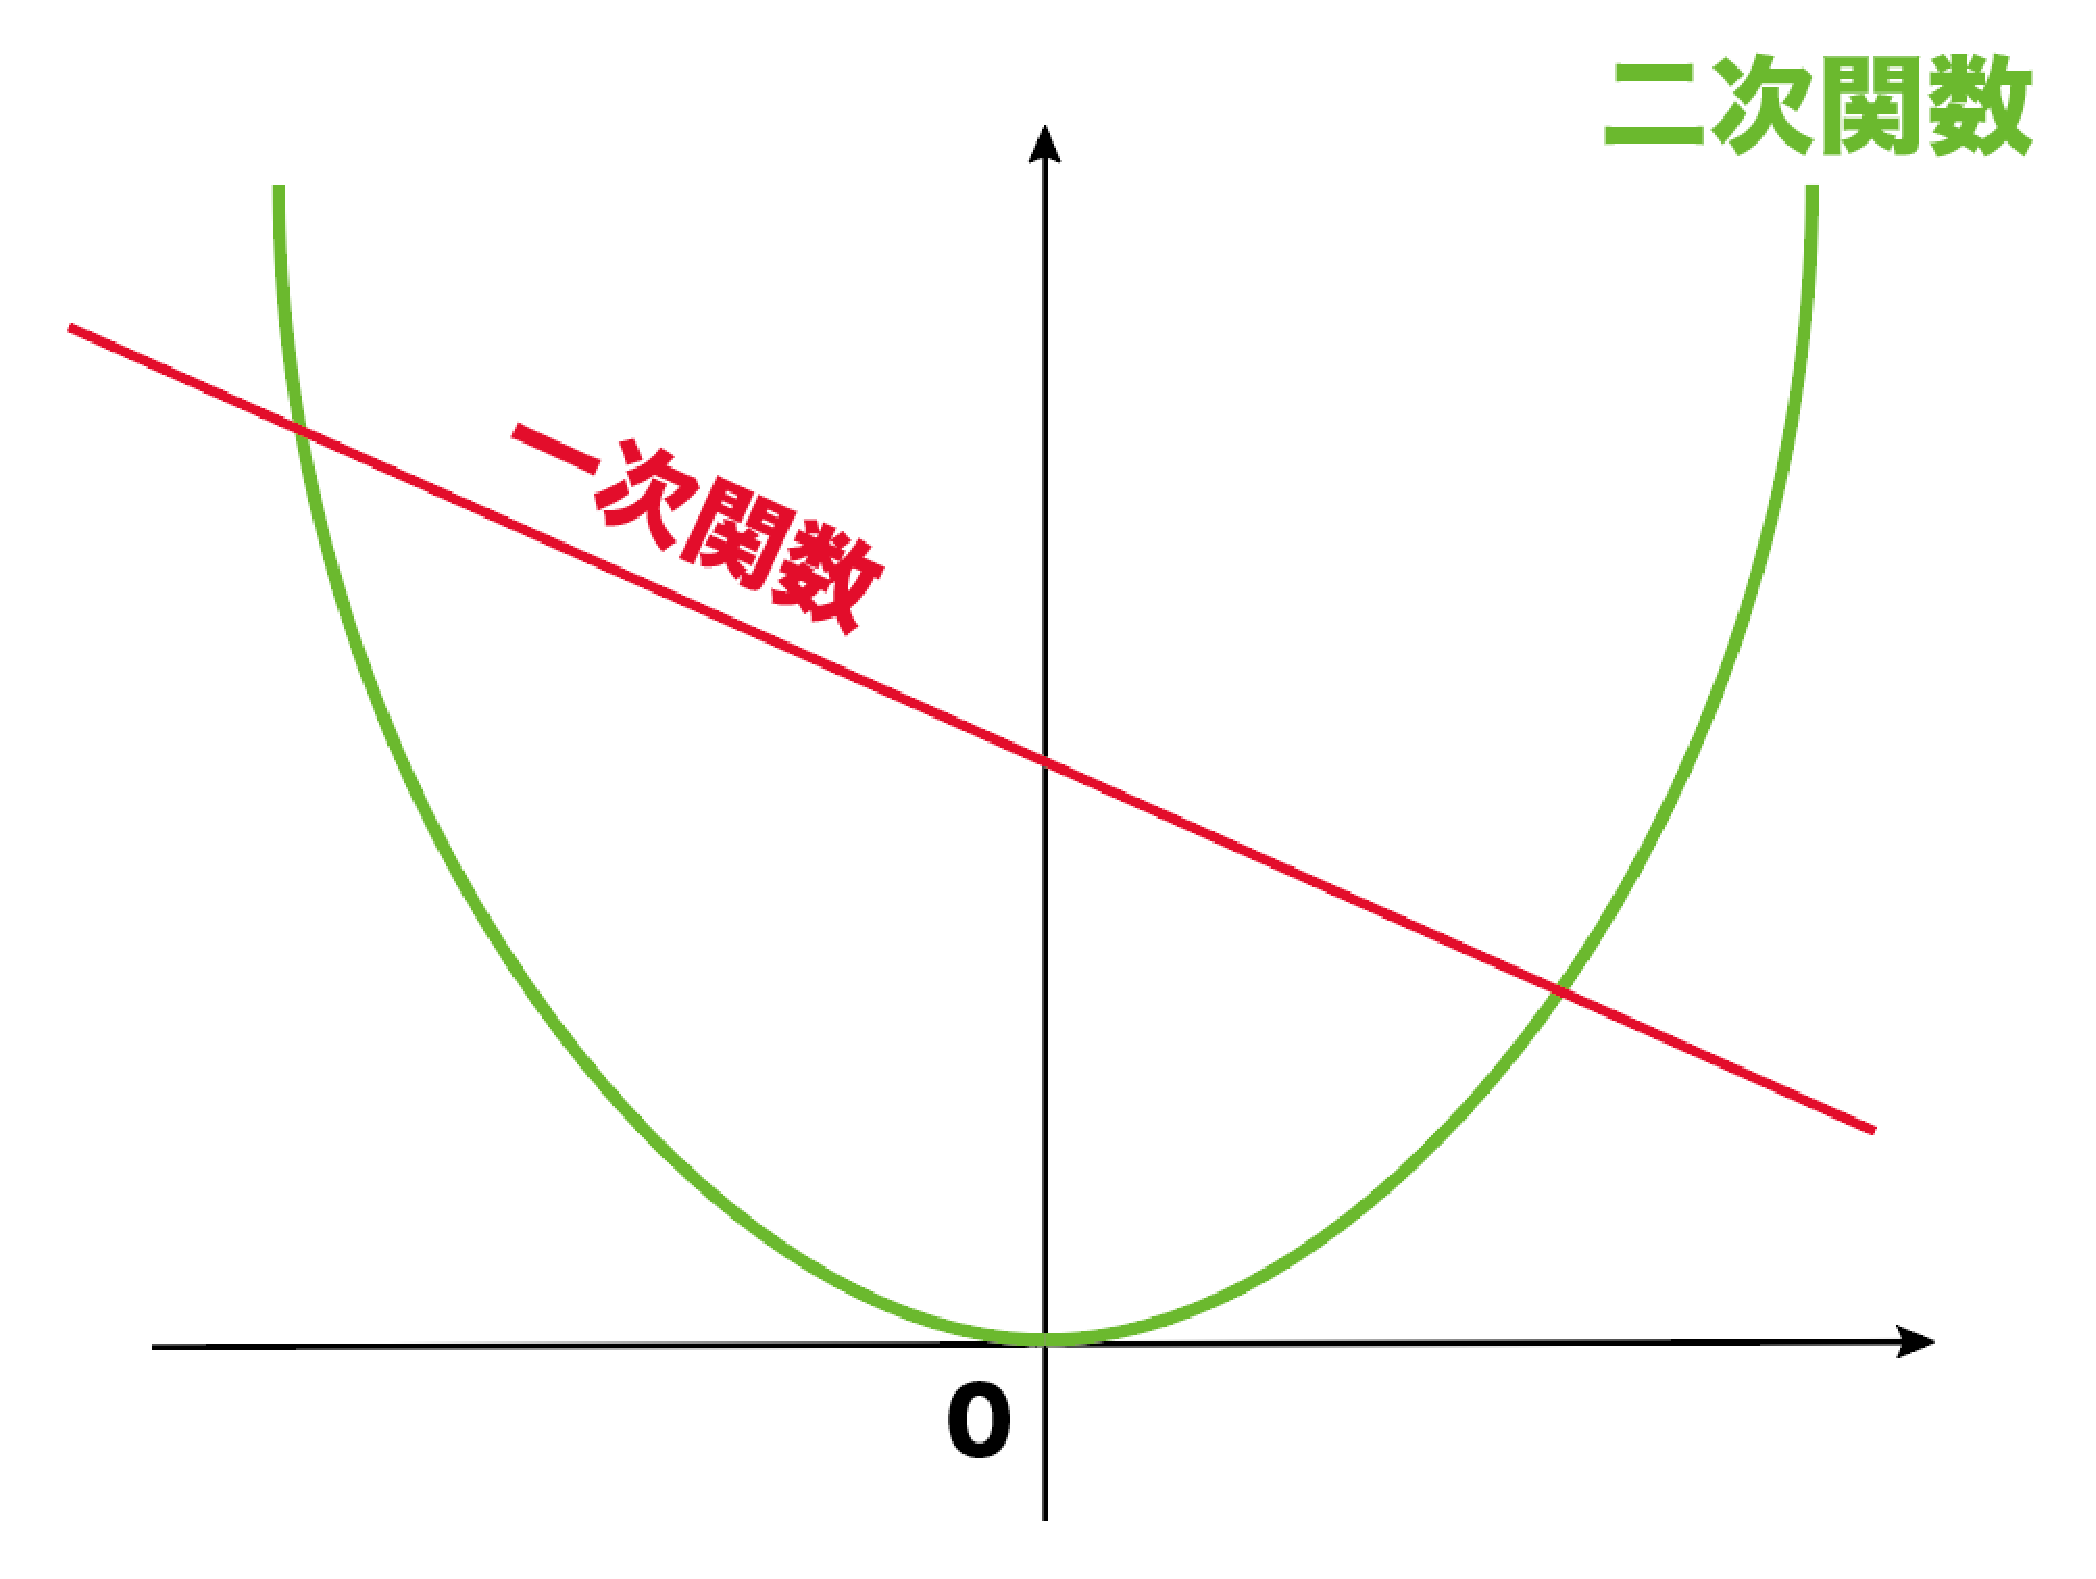
\includegraphics[clip,width=3.5cm]{figure/fig1.eps}
        \caption{title}
        \label{fig:label1}
      \end{center}
    \end{minipage}
    
    \begin{minipage}{0.24\hsize}
      \begin{center}
        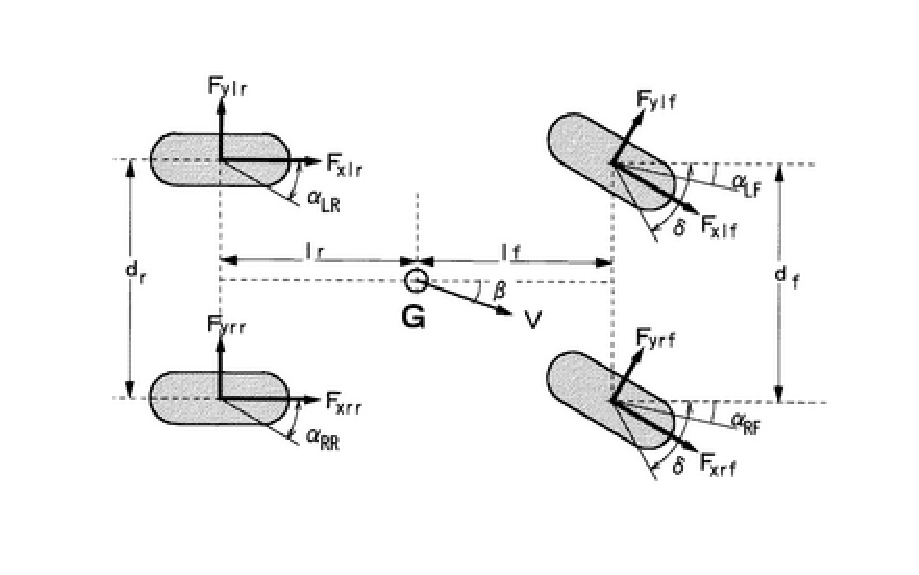
\includegraphics[clip,width=3.5cm]{figure/fig2.eps}
        \caption{title}
        \label{fig:label2}
      \end{center}
    \end{minipage}
    
    %% \begin{minipage}{0.24\hsize}
    %%   \begin{center}
    %%     \includegraphics[clip,width=3.5cm]{figure/fig3.eps}
    %%     \caption{title}
    %%     \label{fig:label3}
    %%   \end{center}
    %% \end{minipage}
    
    %% \begin{minipage}{0.24\hsize}
    %%   \begin{center}
    %%     \includegraphics[clip,width=3.5cm]{figure/fig4.eps}
    %%     \caption{title}
    %%     \label{fig:label4}
    %%   \end{center}
    %% \end{minipage}
    
  \end{tabular}
\end{figure}  

\begin{figure}[H]
  \begin{tabular}{cccc}
    
    %% \begin{minipage}{0.24\hsize}
    %%   \begin{center}
    %%     \includegraphics[clip,width=3.5cm]{figure/fig5.eps}
    %%     \caption{title}
    %%     \label{fig:label5}
    %%   \end{center}
    %% \end{minipage}
    
    %% \begin{minipage}{0.24\hsize}
    %%   \begin{center}
    %%     \includegraphics[clip,width=3.5cm]{figure/fig6.eps}
    %%     \caption{title}
    %%     \label{fig:label6}
    %%   \end{center}
    %% \end{minipage}
    
    %% \begin{minipage}{0.24\hsize}
    %%   \begin{center}
    %%     \includegraphics[clip,width=3.5cm]{figure/fig7.eps}
    %%     \caption{title}
    %%     \label{fig:label7}
    %%   \end{center}
    %% \end{minipage}
    
    %% \begin{minipage}{0.24\hsize}
    %%   \begin{center}
    %%     \includegraphics[clip,width=3.5cm]{figure/fig8.eps}
    %%     \caption{title}
    %%     \label{fig:label8}
    %%   \end{center}
    %% \end{minipage}
    
  \end{tabular}
\end{figure}  

\begin{figure}[H]
  \begin{tabular}{cccc}
    
    %% \begin{minipage}{0.24\hsize}
    %%   \begin{center}
    %%     \includegraphics[clip,width=3.5cm]{figure/fig9.eps}
    %%     \caption{title}
    %%     \label{fig:label9}
    %%   \end{center}
    %% \end{minipage}
    
    %% \begin{minipage}{0.24\hsize}
    %%   \begin{center}
    %%     \includegraphics[clip,width=3.5cm]{figure/fig10.eps}
    %%     \caption{title}
    %%     \label{fig:label10}
    %%   \end{center}
    %% \end{minipage}
    
    %% \begin{minipage}{0.24\hsize}
    %%   \begin{center}
    %%     \includegraphics[clip,width=3.5cm]{figure/fig11.eps}
    %%     \caption{title}
    %%     \label{fig:label11}
    %%   \end{center}
    %% \end{minipage}
    
    %% \begin{minipage}{0.24\hsize}
    %%   \begin{center}
    %%     \includegraphics[clip,width=3.5cm]{figure/fig12.eps}
    %%     \caption{title}
    %%     \label{fig:label12}
    %%   \end{center}
    %% \end{minipage}
    
  \end{tabular}
\end{figure}  

\begin{figure}[H]
  \begin{tabular}{cccc}
    
    %% \begin{minipage}{0.24\hsize}
    %%   \begin{center}
    %%     \includegraphics[clip,width=3.5cm]{figure/fig13.eps}
    %%     \caption{title}
    %%     \label{fig:label13}
    %%   \end{center}
    %% \end{minipage}
    
    %% \begin{minipage}{0.24\hsize}
    %%   \begin{center}
    %%     \includegraphics[clip,width=3.5cm]{figure/fig14.eps}
    %%     \caption{title}
    %%     \label{fig:label14}
    %%   \end{center}
    %% \end{minipage}
    
    %% \begin{minipage}{0.24\hsize}
    %%   \begin{center}
    %%     \includegraphics[clip,width=3.5cm]{figure/fig15.eps}
    %%     \caption{title}
    %%     \label{fig:label15}
    %%   \end{center}
    %% \end{minipage}
    
    %% \begin{minipage}{0.24\hsize}
    %%   \begin{center}
    %%     \includegraphics[clip,width=3.5cm]{figure/fig6.eps}
    %%     \caption{title}
    %%     \label{fig:label16}
    %%   \end{center}
    %% \end{minipage}
    
  \end{tabular}
\end{figure}  

\begin{figure}[H]
  \begin{tabular}{cccc}
    
    %% \begin{minipage}{0.24\hsize}
    %%   \begin{center}
    %%     \includegraphics[clip,width=3.5cm]{figure/fig17.eps}
    %%     \caption{title}
    %%     \label{fig:label17}
    %%   \end{center}
    %% \end{minipage}
    
    %% \begin{minipage}{0.24\hsize}
    %%   \begin{center}
    %%     \includegraphics[clip,width=3.5cm]{figure/fig18.eps}
    %%     \caption{title}
    %%     \label{fig:label18}
    %%   \end{center}
    %% \end{minipage}
    
    %% \begin{minipage}{0.24\hsize}
    %%   \begin{center}
    %%     \includegraphics[clip,width=3.5cm]{figure/fig19.eps}
    %%     \caption{title}
    %%     \label{fig:label19}
    %%   \end{center}
    %% \end{minipage}
    
    %% \begin{minipage}{0.24\hsize}
    %%   \begin{center}
    %%     \includegraphics[clip,width=3.5cm]{figure/fig20.eps}
    %%     \caption{title}
    %%     \label{fig:label20}
    %%   \end{center}
    %% \end{minipage}
    
  \end{tabular}
\end{figure}  

\begin{figure}[H]
  \begin{tabular}{cccc}
    
    %% \begin{minipage}{0.24\hsize}
    %%   \begin{center}
    %%     \includegraphics[clip,width=3.5cm]{figure/fig21.eps}
    %%     \caption{title}
    %%     \label{fig:label21}
    %%   \end{center}
    %% \end{minipage}
    
    %% \begin{minipage}{0.24\hsize}
    %%   \begin{center}
    %%     \includegraphics[clip,width=3.5cm]{figure/fig22.eps}
    %%     \caption{title}
    %%     \label{fig:label22}
    %%   \end{center}
    %% \end{minipage}
    
    %% \begin{minipage}{0.24\hsize}
    %%   \begin{center}
    %%     \includegraphics[clip,width=3.5cm]{figure/fig23.eps}
    %%     \caption{title}
    %%     \label{fig:label23}
    %%   \end{center}
    %% \end{minipage}
    
    %% \begin{minipage}{0.24\hsize}
    %%   \begin{center}
    %%     \includegraphics[clip,width=3.5cm]{figure/fig24.eps}
    %%     \caption{title}
    %%     \label{fig:label24}
    %%   \end{center}
    %% \end{minipage}
    
  \end{tabular}
\end{figure}  

\begin{figure}[H]
  \begin{tabular}{cccc}
    
    %% \begin{minipage}{0.24\hsize}
    %%   \begin{center}
    %%     \includegraphics[clip,width=3.5cm]{figure/fig25.eps}
    %%     \caption{title}
    %%     \label{fig:label25}
    %%   \end{center}
    %% \end{minipage}
    
    %% \begin{minipage}{0.24\hsize}
    %%   \begin{center}
    %%     \includegraphics[clip,width=3.5cm]{figure/fig26.eps}
    %%     \caption{title}
    %%     \label{fig:label26}
    %%   \end{center}
    %% \end{minipage}
    
    %% \begin{minipage}{0.24\hsize}
    %%   \begin{center}
    %%     \includegraphics[clip,width=3.5cm]{figure/fig27.eps}
    %%     \caption{title}
    %%     \label{fig:label27}
    %%   \end{center}
    %% \end{minipage}
    
    %% \begin{minipage}{0.24\hsize}
    %%   \begin{center}
    %%     \includegraphics[clip,width=3.5cm]{figure/fig28.eps}
    %%     \caption{title}
    %%     \label{fig:label28}
    %%   \end{center}
    %% \end{minipage}
    
  \end{tabular}
\end{figure}

\end{document}
